%%%%%%%%%%%%%%%%%%%%%%%%%%%%%%%%%%%%%%%%%
% Beamer Presentation
% LaTeX Template
% Version 1.0 (10/11/12)
%
% This template has been downloaded from:
% http://www.LaTeXTemplates.com
%
% License:
% CC BY-NC-SA 3.0 (http://creativecommons.org/licenses/by-nc-sa/3.0/)
%
%%%%%%%%%%%%%%%%%%%%%%%%%%%%%%%%%%%%%%%%%

%----------------------------------------------------------------------------------------
%	PACKAGES AND THEMES
%----------------------------------------------------------------------------------------

\documentclass{beamer}
\usepackage[utf8]{inputenc}
\usepackage[portuguese]{babel}
\mode<presentation> {

% The Beamer class comes with a number of default slide themes
% which change the colors and layouts of slides. Below this is a list
% of all the themes, uncomment each in turn to see what they look like.

%\usetheme{default}
%\usetheme{AnnArbor}
%\usetheme{Antibes}
%\usetheme{Bergen}
%\usetheme{Berkeley}
%\usetheme{Berlin}
%\usetheme{Boadilla}
%\usetheme{CambridgeUS}
%\usetheme{Copenhagen}
%\usetheme{Darmstadt}
%\usetheme{Dresden}
%\usetheme{Frankfurt}
%\usetheme{Goettingen}
%\usetheme{Hannover}
\usetheme{Ilmenau}
%\usetheme{JuanLesPins}
%\usetheme{Luebeck}
%\usetheme{Madrid}
%\usetheme{Malmoe}
%\usetheme{Marburg}
%\usetheme{Montpellier}
%\usetheme{PaloAlto}
%\usetheme{Pittsburgh}
%\usetheme{Rochester}
%*\usetheme{Singapore}
%\usetheme{Szeged}
%\usetheme{Warsaw}

% As well as themes, the Beamer class has a number of color themes
% for any slide theme. Uncomment each of these in turn to see how it
% changes the colors of your current slide theme.

%\usecolortheme{albatross}
% Mesma cor do trabalho original
%\usecolortheme{beaver}
%\usecolortheme{beetle}
%\usecolortheme{crane}
%\usecolortheme{dolphin}
%\usecolortheme{dove}
%\usecolortheme{fly}
%\usecolortheme{lily}
%\usecolortheme{orchid}
%\usecolortheme{rose}
%\usecolortheme{seagull}
%\usecolortheme{seahorse}
\usecolortheme{whale}
%\usecolortheme{wolverine}

%\setbeamertemplate{footline} % To remove the footer line in all slides uncomment this line
\setbeamertemplate{footline}[page number] % To replace the footer line in all slides with a simple slide count uncomment this line

%\setbeamertemplate{navigation symbols}{} % To remove the navigation symbols from the bottom of all slides uncomment this line
}
\usepackage{caption}
\usepackage{graphicx} % Allows including images
\usepackage{booktabs} % Allows the use of \toprule, \midrule and \bottomrule in tables

%----------------------------------------------------------------------------------------
%	TITLE PAGE
%----------------------------------------------------------------------------------------

\title{Esteganografia em Imagens Médicas} % The short title appears at the bottom of every slide, the full title is only on the title page

\author{} % Your name
\institute[USP] % Your institution as it will appear on the bottom of every slide, may be shorthand to save space
{
 \\ % Your institution for the title page
\medskip
\textit{} % Your email address
}
\date{} % Date, can be changed to a custom date

\AtBeginSection[]
{
\begin{frame}
\frametitle{}
\tableofcontents[currentsection]
\end{frame}
}

\begin{document}

\begin{frame}
\titlepage % Print the title page as the first slide
\end{frame}
\begin{frame}
Autor: Rafael de Assunção Sampaio

Orientador: Marcel Jackowski

\begin{flushright}
 Eduardo Bier
 
 Fernanda Camargo

 Florence Alyssa

 Marcello Oliveira

 Shayenne Moura
 \end{flushright} % Print the title page as the first slide
\end{frame}
%\begin{frame}
%\frametitle{Visão Geral} % Table of contents slide, comment this block out to remove it
%\tableofcontents % Throughout your presentation, if you choose to use \section{} and \subsection{} commands, these will automatically be printed on this slide as an overview of your presentation
%\end{frame}

%----------------------------------------------------------------------------------------
%	PRESENTATION SLIDES
%----------------------------------------------------------------------------------------

%------------------------------------------------
\section{Introdução} 
%------------------------------------------------

\begin{frame}
\frametitle{Motivação}
\begin{itemize}
\item Confiabilidade dos exames médicos \newline
\item Exposição de dados confidenciais \newline
\item Risco de fraude \newline
\item Garantia de autenticidade
\end{itemize}

\end{frame}

%------------------------------------------------

%------------------------------------------------

\section{DICOM}
%------------------------------------------------
%\subsection{Formato}
\begin{frame}
\frametitle{Descrição do DICOM}

\begin{itemize}
\item \textit{Digital Imaging Communications in Medicine}\newline
\item ACR e NEMA\newline
\item Cabeçalho com informações e matriz da imagem\newline
\end{itemize}
\end{frame}


\begin{frame}
\frametitle{Algumas \textit{tags} DICOM}
\begin{figure}  
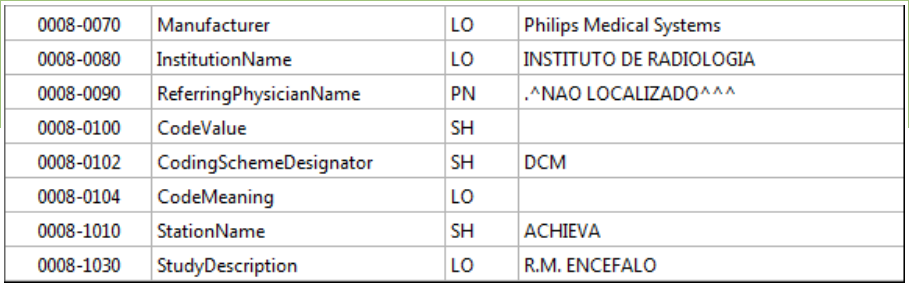
\includegraphics[scale=.3]{table.png} 


\centering{Fonte: Rafael Sampaio, 2012}
\end{figure}
\end{frame}
%------------------------------------------------
%\subsection{Falhas}
\begin{frame}
\frametitle{Falhas do DICOM}

\begin{itemize}
\item Falta de proteção aos dados\newline
\item Passível de modificação\newline
\item Inautenticidade das informações
\end{itemize}

\end{frame}
%------------------------------------------------
\section{Esteganografia}
%\subsection{Definição}

\begin{frame}
\frametitle{Definição}
\begin{itemize}
\item Método de comunicação secreta \newline
\item Mensagem oculta em outra \newline
\item Transmissão indetectável para terceiros


\end{itemize}
\end{frame}

%------------------------------------------------
%\subsection{Origem}
\begin{frame}
\frametitle{Origem}
\begin{itemize}
\item \textit{Steganos}: encoberto \newline
\item \textit{Graphia}: escrita\newline
\item Johannes Trithemius 
\end{itemize}
\end{frame}

%------------------------------------------------
%\subsection{Criptografia $\times$ Esteganografia}
\begin{frame}
\frametitle{Criptografia $\times$ Esteganografia}
\begin{itemize}
\item Semelhança: preocupação com a mensagem \newline
\item Diferença: canal de comunicação
\end{itemize}
\end{frame}

%------------------------------------------------

\begin{frame}
\frametitle{Exemplos de Utilização}
\begin{itemize}
\item Heródoto - história de Aristágoras (V a.C.)\newline
\item Viktor Korchnoi e Anatoly Karpov - Campeonato de xadrez (XX d.C.)\newline
\item Dhiren Barot - Die Hard: With a Vengeance (XXI d.C.)\newline
\end{itemize}
\end{frame}


%------------------------------------------------
%------------------------------------------------
\section{Técnicas de Esteganografia}
%------------------------------------------------
%\subsection{LSB}
\begin{frame}
\frametitle{Bits Menos Significativos -- BMS}

\begin{itemize}
\item Utilização de matriz de tons cinza\newline
\item Alteração pouco perceptível\newline
\item Modificação do bit menos significativo

\end{itemize}

\end{frame}
%------------------------------------------------
\begin{frame}
\frametitle{Análise do BMS}

\begin{itemize}
\item Transformações geométricas\newline
\item Filtros\newline
\item Esquemas de compressão\newline
\item Fácil recuperação dos dados
\end{itemize}

\end{frame}
%------------------------------------------------
%\subsection{DBAM}
\begin{frame}
\frametitle{Divisão em Blocos e Alteração da Média -- DBAM}

\begin{itemize}
\item Divisão da imagem em blocos \newline
\item Cálculo a melhor posição para as alterações\newline
\item Busca da mínima degradação 
\end{itemize}
\end{frame}

%------------------------------------------------
\begin{frame}
\frametitle{Análise do DBAM}

\begin{itemize}
\item Alteração visível \newline
\item Pré-processamento da imagem \newline
\end{itemize}
\end{frame}

%------------------------------------------------

%\subsection{MAMM}
\begin{frame}
\frametitle{Método de Alteração da Média Modificado -- MAMM}

\begin{itemize}
\item Aperfeiçoamento do método anterior \newline
\item Embaralhamento de \textit{pixels} (\textit{shuffling}) \newline
\item Equilíbrio dos tons
\end{itemize}

\end{frame}

%------------------------------------------------
\begin{frame}
\frametitle{Análise do MAMM}

\begin{itemize}
\item Combate dos pontos fracos dos outros métodos \newline
\item Modificação pouco perceptível \newline
\item Eficácia baseada em amostragem
\end{itemize}

\end{frame}

%------------------------------------------------

\section{Resultados}
\begin{frame}
\frametitle{Esteganografia com BMS}
\begin{figure}
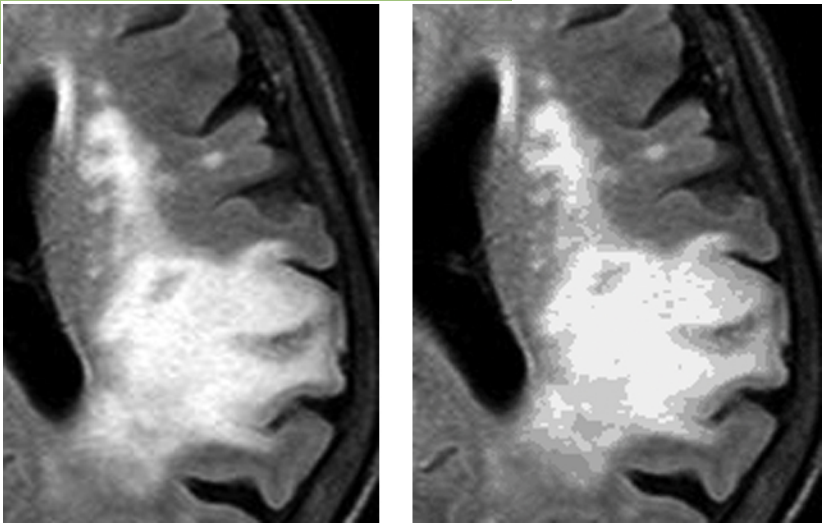
\includegraphics[scale=.2]{BMS.png} 
\caption{À esquerda, imagem original. À direita, após BMS}

\centering{Fonte: Rafael Sampaio, 2012}
\end{figure}
\end{frame}
%------------------------------------------------
\begin{frame}
\frametitle{Esteganografia com BMS}
\begin{figure}
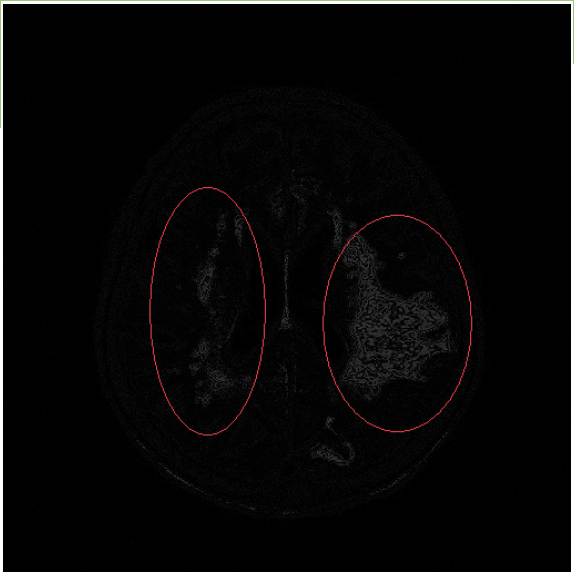
\includegraphics[scale=.2]{BMSdiff.png} 
\caption{Diferença entre as imagens com BMS}

\centering{Fonte: Rafael Sampaio, 2012}
\end{figure}
\end{frame}
%------------------------------------------------
\begin{frame}
\frametitle{Esteganografia com DBAM}
\begin{figure}
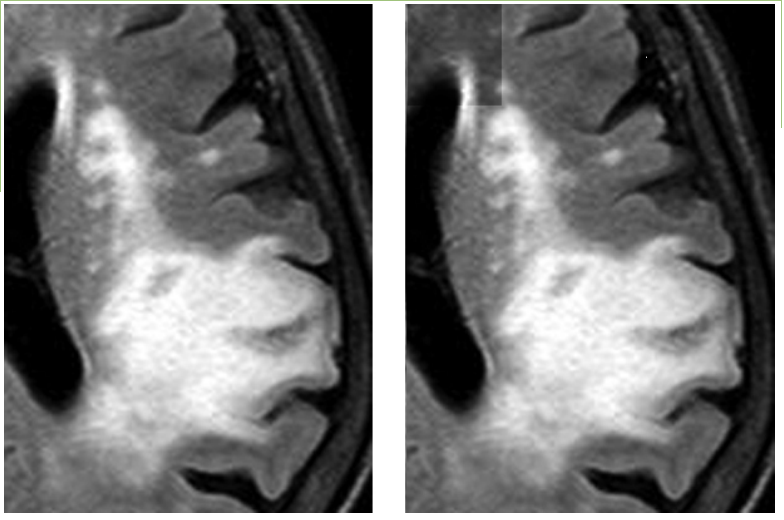
\includegraphics[scale=.2]{DBAM.png} 
\caption{À esquerda, imagem original. À direita, após DBAM}

\centering{Fonte: Rafael Sampaio, 2012}
\end{figure}
\end{frame}
%------------------------------------------------
\begin{frame}
\frametitle{Esteganografia com DBAM}
\begin{figure}

\includegraphics[scale=.2]{DBAMdiff.png} 
\caption{Diferença entre as imagens com DBAM}

\centering{Fonte: Rafael Sampaio, 2012}
\end{figure}
\end{frame}
%------------------------------------------------
\begin{frame}
\frametitle{Esteganografia com MAMM}
\begin{figure}
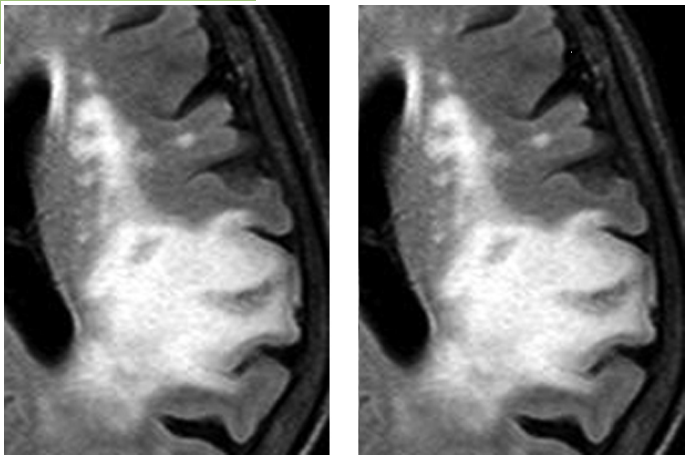
\includegraphics[scale=.2]{MAMM.png} 
\caption{À esquerda, imagem original. À direita, após MAMM}

\centering{Fonte: Rafael Sampaio, 2012}
\end{figure}
\end{frame}

%------------------------------------------------
\begin{frame}
\frametitle{Esteganografia com MAMM}
\begin{figure}

\includegraphics[scale=.2]{MAMMdiff.png} 
\caption{Diferença entre as imagens com MAMM}

\centering{Fonte: Rafael Sampaio, 2012}
\end{figure}
\end{frame}

%------------------------------------------------
\section{Conclusões}
\begin{frame}[fragile] % Need to use the fragile option when verbatim is used in the slide
\frametitle{Conclusões}
\begin{itemize}

\item Utilização do DICOM e o sigilo dos dados\newline

\item Eficácia do Método de Alteração das Médias Modificado \newline

\item Integração MAMM e DICOM \newline

\end{itemize}
\end{frame}

\end{document}
